%!TeX program = xelatex
\documentclass[12pt,hyperref,a4paper,UTF8]{ctexart}
\usepackage{SJTUReport}
\usepackage{url}
\setcounter{biburllcpenalty}{7000}
\setcounter{biburlucpenalty}{8000}

%%-------------------------------正文开始---------------------------%%
\begin{document}
	
	%%-----------------------封面--------------------%%
	\cover
	
	%%------------------摘要-------------%%
	\begin{abstract}
	
	本次大作业基于Qwen2.5-Math-1.5B模型进行实验,主要包括SFT和GRPO两部分的内容。在实验中,我们补全了GRPO部分的reward计算和loss计算,并修改了SFT和evaluation的代码,使得可以高效地实验不同超参数对short cot sft的影响。实验结果表明,我们的方法在多个数据集上取得了优于baseline的表现,long cot、grpo严格优于baseline,short cot和baseline相当。
	
	\end{abstract}
	
	\thispagestyle{empty} % 首页不显示页码
	
	%%--------------------------目录页------------------------%%
	\newpage
	\tableofcontents
	
	%%------------------------正文页从这里开始-------------------%
	\newpage
	\section{SFT}
	本节介绍基于Qwen2.5-Math-1.5B模型的SFT实验,包括short cot和long cot两种方式。
	
	\subsection{Short COT}
	在short cot实验中,我们修改了原有代码,使其能够高效地实验不同超参数对训练效果的影响。实验结果显示,部分指标超过了short cot sft baseline。
	
	由于Short CoT的参数调节较为复杂,因此需要对可能的状态空间进行搜索
	
	首先进行粗略搜索,状态空间为:
	\begin{lstlisting}[language=python]
evaluation_epochs = [3, 6]
explore_batch_size = [128, 256, 512]
explore_lr = [1e-5, 2e-5, 4e-5]
	\end{lstlisting}
	按照4个指标相对baseline比值的调和平均数(会放大最小值的影响)作为评价分数得到的结果如图~\ref{fig:pic1}所示。
	\begin{figure}[htbp]
		\centering
		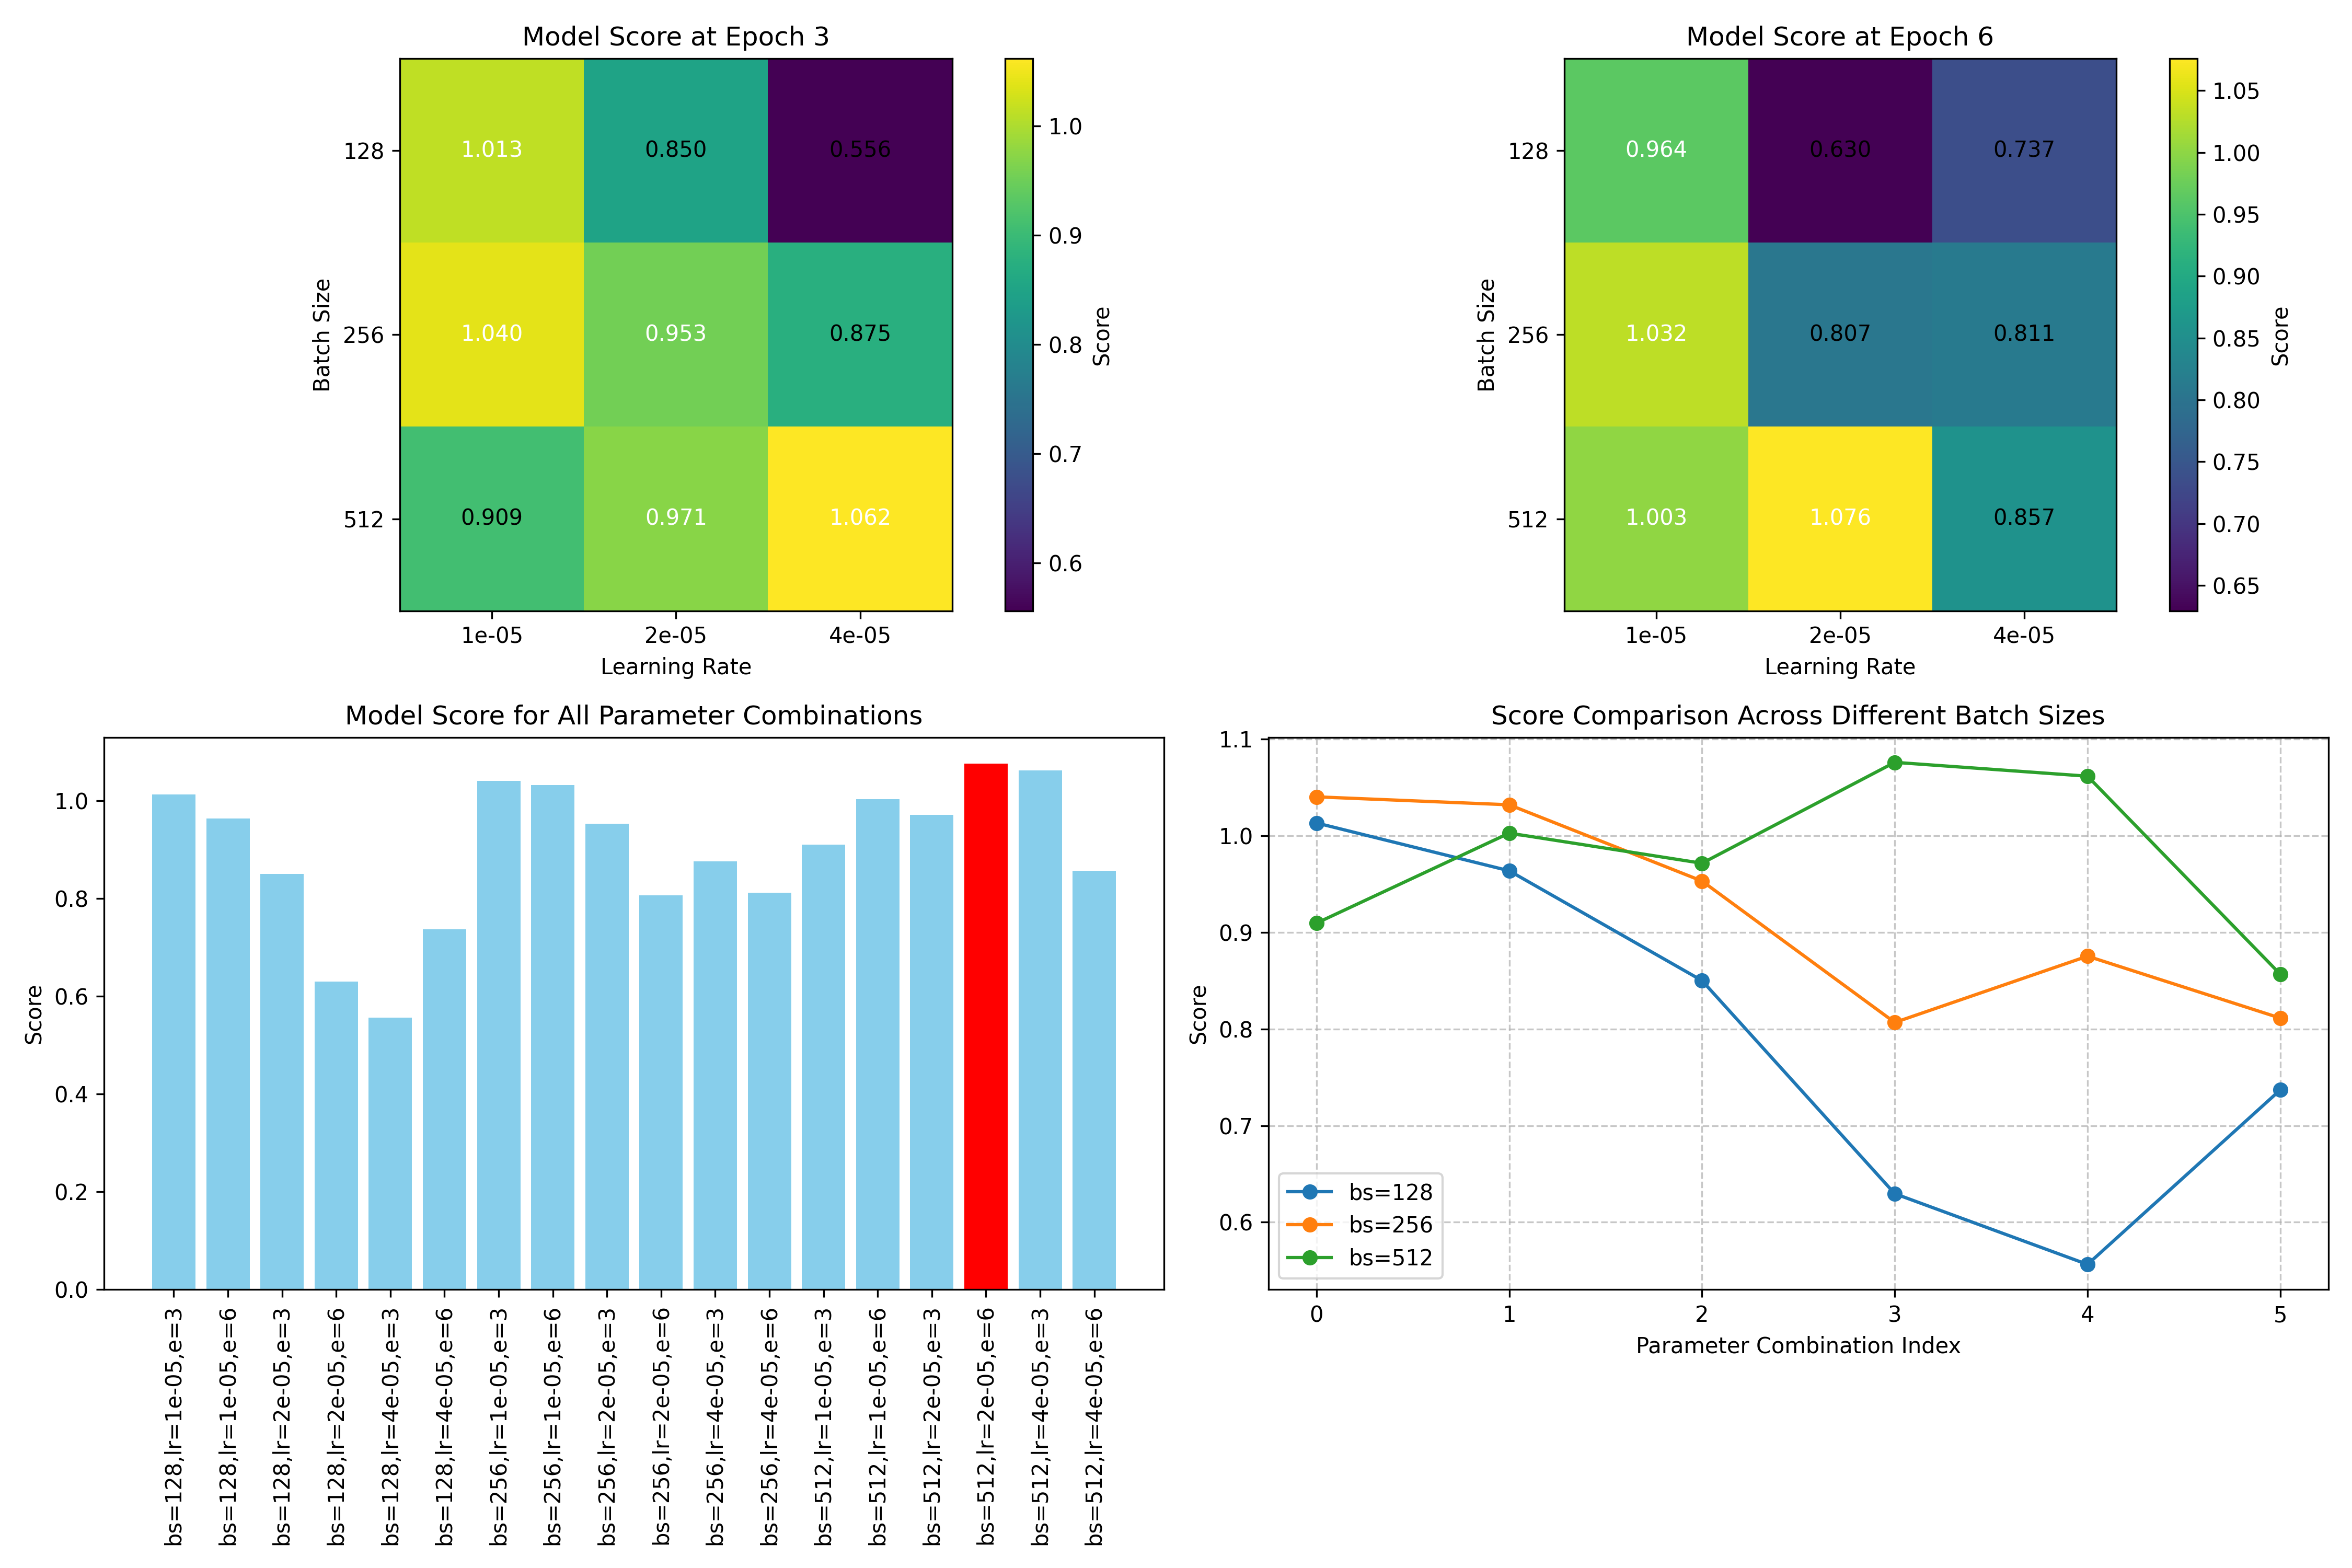
\includegraphics[width=\textwidth]{pic1.png}
		\caption{short cot sft 超参数第一轮搜索}
		\label{fig:pic1}
	\end{figure}
	第一轮得到的最大值: 1.0758890919394155, 对应的参数: (512, 2e-05, 6),具体表现如下:
	\begin{itemize}
		\item AMC23 acc: 0.4
		\item GSM8k acc: 0.707
		\item MATH500 acc: 0.412
		\item OlympiadBench acc: 0.108
	\end{itemize}
	其中有2个指标严格大于baseline,1个指标略小于baseline,1个指标小于baseline,考虑到正确率比值的调和平均值$1.07>1$,可以认为这个模型的能力和baseline近似相当。
	
	\subsection{Long COT}
	在long cot实验中,我们的模型在所有指标上全部超过了long cot sft baseline,具体表现如下:
	\begin{itemize}
		\item AMC23 acc: 0.325
		\item GSM8k acc: 0.694
		\item MATH500 acc: 0.408
		\item OlympiadBench acc: 0.138
	\end{itemize}
	
	训练参数设置为:BS=128, EP=6, LR=2e-5。
	
	\section{GRPO}
	本节介绍基于Qwen2.5-Math-1.5B模型的GRPO实验。我们的方法在所有指标上全部超过了grpo baseline,具体表现如下:
	\begin{itemize}
		\item AMC23 acc: 0.525
		\item GSM8k acc: 0.775
		\item MATH500 acc: 0.618
		\item OlympiadBench acc: 0.246
	\end{itemize}
	
	\subsection{训练流程}
	整个训练的流程是在GRPO的基础上进行人工划分阶段的curriculum learning,主要分为基本训练和质量提升训练两个阶段。超参数是直接使用框架里给的超参数。
	\subsubsection{相关探索}
	\begin{itemize}
		\item 修改题目的难度配比:几乎没有效果,甚至有负面影响
		\item 从sft的结果开始训练:几乎没有效果
		\item 使用DAPO的论文\cite{yu_DAPOOpenSourceLLM_2025}里提到的Clip-Higher:有效果
	\end{itemize}
	\subsubsection{基本训练}
	在基本训练阶段,我们使用默认数据集和默认LOSS函数,设计了如下reward函数:
	\begin{itemize}
		\item 回答无法解析出答案:-1
		\item 答案错误:0
		\item 答案正确:100
	\end{itemize}
	基本训练过程分为3轮,每一轮结束后,人工通过reward等指标的变化判断“最有潜力”的checkpoint最为下一轮的训练起点。
	
	\subsubsection{质量提升训练}
	在质量提升训练阶段,我们使用默认数据集和默认LOSS函数,设计了更为复杂的reward函数:
	\begin{itemize}
		\item 回答无法解析出答案:-10
		\item 答案错误:0
		\item 答案正确:100
		\item 思维链长度bonus:在回答中没有重复的情况下,提供一个不超过10的长度bonus
		\item 语言bonus:不出现中英混杂的情况时,可获得5分的bonus
	\end{itemize}
	质量提升训练共2轮,其中第2轮打开了Clip-Higher。
	
	\newpage
	\appendix
	%%----------- 参考文献 -------------------%%
	%在reference.bib文件中填写参考文献,此处自动生成
	\section{如何复现与具体代码、数据}
	仓库地址:\url{https://github.com/happyZYM/cs2916-2025},实验日志:\url{https://wandb.ai/zymx/cs2916-2025}
	\begin{itemize}
		\item shortcot: 运行\textit{scripts/explore.py},或者直接用对应超参数训练。效果可能有一定差别。
		\item longcot: 运行\textit{scripts/sft\_longcot.sh}。效果可能有一定差别。
		\item grpo:无法一键复现,请根据前文讲述的过程调节\textit{scripts/grpo.sh}、reward、loss相关代码。同时,由于RL的随机性相当大,不保证效果能完全达到前文所述的效果,验证请从后文的链接下载checkpoint进行验证。
	\end{itemize}
	short COT、long cot、grpo三部分训练出的模型checkpoint可以通过以下方式下载:

	\begin{itemize}
		\item 交大云盘:链接\url{https://pan.sjtu.edu.cn/web/share/860110312f97f0a9673f0f2dc050644c},提取码: uqrz
		\item 备用下载方式:
		\begin{itemize}
			\item shortcot sft:\url{https://alist-cf.zhuangyumin.dev/x/share/cs2916-2025-hw1/sft_shortcot_512_2e-5_6.tar.zst?sign=DVfROmggJ0rchjSJJhM8HgnK_9cK8LkXgXX_ASMkny4=:0}
			\item longcot sft:\url{https://alist-cf.zhuangyumin.dev/x/share/cs2916-2025-hw1/sft_longcot5.tar.zst?sign=JQmlhJpzXMF87NaLvVEluwUwYGX7vuHJsMzcfryUnyY=:0}
			\item grpo: \url{https://alist-cf.zhuangyumin.dev/x/share/cs2916-2025-hw1/grpo_quality_round2.tar.zst?sign=4ftP-CJSHMHLSlCZkD8cj4ZltxQBZvkNxSjEhHXjCxo=:0}
		\end{itemize}
	\end{itemize}
	\section{REFERENCES}
	\nocite{*}
	\printbibliography[heading=none]
	
	
\end{document}